\ofsubsection{Combat}
%
\ofquote{"Enough expository banter. It's time we fight like men. And ladies. And ladies who dress like men."\\}{Gilgamesh}\\
%
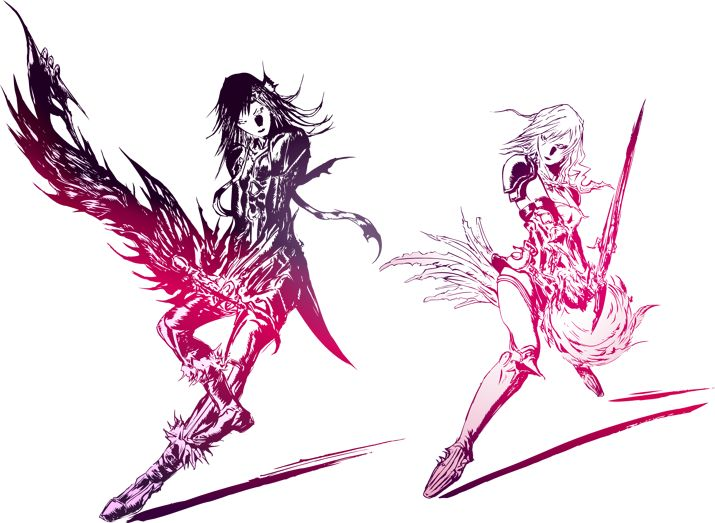
\includegraphics[width=\columnwidth]{./art/images/ff13-2.jpg}
%
\vfill
%
\accf{Combat} consists of a series of rounds (shortened~\accf{r}) that take 10 seconds of in-game time each.
During a round, each combatant takes one turn.
At the start of the battle, both parties choose who takes the first turn in each round on their side.
The GM then decides which side goes first.
At the end of every turn, select an ally who has not taken a turn in this round and takes the next turn for your side.
Both sides take alternating turns until everyone has taken one and the round is completed.
The GM should announce the start and end of each round to avoid confusion.
If one side has more combatants than the other, they take consecutive turns at the end of the round until everyone has taken a turn.
When a party ambushes the other before combat, the GM can decide that they gain a \accf{surprise round}.
In this case, only the surprising party acts in the first round before the battle continues as usual.
%
\vfill
%
Combat proficiencies are determined by the following 7 numerical \accf{attributes}.
Whenever a calculation results in a non-integer value, the result is always rounded down.
%
\ofgap
%
\newcommand{\attricon}[1]{\raisebox{-.15\height}{\includegraphics[height=0.8\baselineskip]{./art/icons/#1.png}}\hspace*{0.15cm}}
%
\attricon{hp}\accf{Hit Points (HP)} increase your durability. You have a maximum and a current number of HP, if your current HP falls to 0 you fall unconscious. \ofrow
\attricon{mp}\accf{Mana Points (MP)} are the resource required for using abilities such as Magic and Techs. Similar to HP, you have a maximum and a current number of MP. \ofrow
\attricon{str}\accf{Strength (STR)} increases the damage dealt by your physical attacks. \ofrow
\attricon{def}\accf{Defense (DEF)} increases your resilience against physical damage. \ofrow
\attricon{mag}\accf{Magic (MAG)} increases the potency of your healing and attacking spells. \ofrow
\attricon{res}\accf{Resistance (RES)} increases your resilience against magical damage. \ofrow
\attricon{mov}\accf{Agility (AGI)} allows you to evade physical attacks and determines how quickly you can move.
%
\newpage
%
During your turn you can, in any order, move a distance of your AGI+1 units and take an action.
Below is a list of combat actions, but the GM may allow any other action that can be completed in one turn:\ofgap
%
\attricon{attack}\accf{Attack:}
You attack an enemy with your weapon. 
He may evade by passing an \accf{evasion check} with a DC of 12 minus his AGI. 
If he fails the check, you reduce the target's HP by your weapon's DMG plus your STR.
If the evader rolls a 2, you make a \mbox{\accf{critical hit}}, doubling your usual damage. 
If he rolls a 12, not only does your Attack miss, but the evader makes an Attack action on you instead, which you cannot evade.\ofgap
%
\attricon{magic}\accf{Magic:}
You cast a spell by spending MP, choosing a target within its range and concentrating for a duration.
While concentrating, you cannot take actions or evade. 
After the cast time is up, the spell's effect occurs on the target right \accf{before your turn} and cannot be evaded even if you are not in range anymore.
If the spell deals damage or restores HP, add your MAG to the amount.
Every spell's description has information on its cast time, MP cost, target, range and effect.\ofgap
%
\attricon{tech}\accf{Tech:}
You use a non-magical ability. 
Techs are used the same way as magic, but their damage and healing is amplified by your STR instead of your MAG, 
except if their use already includes this bonus in another way, for example by involving an Attack.\ofgap
%
\attricon{defend}\accf{Defend:} All damage that you receive by Attacks until your next turn is halved. \ofgap
%
\attricon{item}\accf{Item:} You use an Item from your inventory on yourself or someone within 1u.\ofgap
%
\accf{Re-Equip:} Swap a Materia or Equipment piece that you are wearing against one from your Inventory.\ofgap
%
\accf{Dash:} Move another distance of your AGI+1 units.\\\\
%
Apart from Magic and Techs, characters can also learn the following \accf{special abilities}: \ofrow
\attricon{passive}\accf{Passive:} Effects that are permanently active. \ofgap
\attricon{react}\accf{Reaction:} Allow you to take certain actions on someone else's turn under specific conditions.
%
\vfill
%
\ofboxwithtitle{Example: Combat}
{
	Squall (4 DEF, 3 AGI, 1 RES) and Seifer (6 STR, 2 MAG) decide to duel.
	Both are wielding a gunblade~(1d DMG) and the GM decides that Seifer takes the first turn.
	He begins casting Firaga (6d DMG, 1r Time) by spending 12~MP, choosing Squall as target and concentrating.
	Squall uses his turn to Defend.
	It's Seifer's turn again, so Firaga takes effect and Squall suffers \mbox{6d+2-1} damage. 
	Seifer can still take his turn, so he also Attacks. 
	Squall makes a \mbox{DC 12-3} evasion check, but by rolling [1, 1] he fails and suffers a Critical Hit! 
	Seifer hits him right above the nose with his blade, inflicting \mbox{1d+6-4} damage (Defend and Critical Hit cancel each other out) and leaving a scar.
}
%
\clearpage
%
\newcommand{\elemicon}[1]{\hspace*{0.15cm}\raisebox{-.2\height}{\includegraphics[height=\baselineskip]{./art/icons/#1.png}}}
%
All damage dealt has one of two basic types.
Damage dealt by Attacks and Techs is usually \accf{physical}. 
When you receive physical damage, subtract your DEF from the amount.
Damage dealt by Magic and Items is usually \accf{magical}. 
When you receive magical damage, subtract your RES from the amount.
In addition, damage can have an elemental type to which combatants can have \accf{Weaknesses} or \accf{Resiliences}. 
When resilient, you only suffer half the usual damage and when weak, you suffer double the usual damage. 
Resilience and Weakness cancel each other out and do not stack.
The following elemental types exist: fire\elemicon{fire}, ice\elemicon{ice}, lightning\elemicon{lightning}, earth\elemicon{earth}, water\elemicon{water}, holy\elemicon{holy} and dark\elemicon{dark}.
%
\vfill
%
\accf{Units} (shortened \accf{u}) are the basis to measure distance, where 1u is roughly 1m or 3ft.
Characters usually occupy a circle of 1u in diameter in top view. 
Effect distances are described by their Range and Target.
\accf{Range} is the maximum distance between the center of the caster and the center of the effect. 
An effect with range Self is centered at the caster, and one with range Weapon has the same range as the used weapon.
\accf{Target} is the area of the effect as a maximum distance from its center. Unless stated otherwise, everyone fully or partially in the target area is affected, including allies.
An effect with target Single affects only a single entity.
The following illustration shows the use of a ranged effect in the normal case and with the two special target shapes Line and Front. 
%
\begin{figure}[h!]
		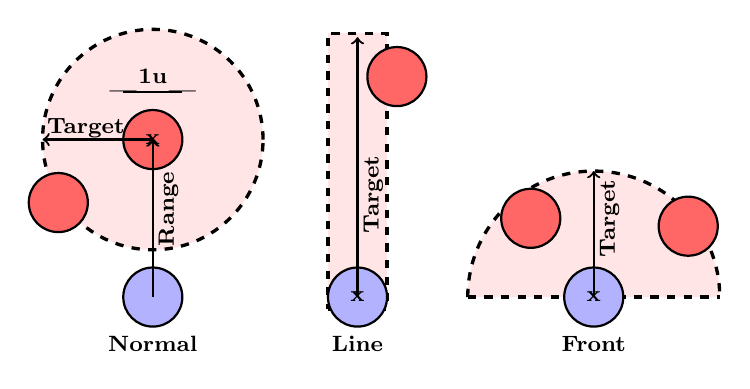
\begin{tikzpicture}[]
		\tikzstyle{test}=[thick, draw, circle, align=center]					
		%Normal
		\node[fill=blue!30!white, test,minimum size = 0.75cm](caster)at (0,0) {};
		\node[](t2)at (0,-0.6) {\bf\footnotesize Normal};
		\node[fill=red!10!white, test, very thick, dashed ,minimum size = 2.8cm](tarea)at (0,2) {};
		\node[fill=red!60!white, test,minimum size = 0.75cm](target)at (0,2) {};
		\node[fill=red!60!white, test,minimum size = 0.75cm](target)at (-1.2,1.2) {};
		\draw[thick, ->](0,0) -- node[] {}(0,2);
		\draw[thick, ->](0,2) -- node[] {}(-1.4, 2);
		\node[rotate=90](t1)at (0.2,1.12) {\bf\footnotesize Range};
		\node[](t2)at (-0.85,2.15) {\bf\footnotesize Target};
		\node[](t3)at (0,2) {\bf\footnotesize x};
		\node[](fi)at (-0.375,2.6) {\bf\footnotesize |};
		\node[](se)at (0.375,2.6) {\bf\footnotesize |};
		\draw[thick, -](0.375,2.6) -- node[] {}(-0.375,2.6);
		\node[](sca)at (0,2.8) {\bf\footnotesize 1u};		
		%Line
		\node[draw, fill=red!10!white, rectangle, very thick, dashed ,minimum height = 3.5cm, minimum width=0.75cm](tarea)at (2.6,1.6) {};
		\node[fill=blue!30!white, test,minimum size = 0.75cm](caster)at (2.6,0) {};
		\node[](t2)at (2.6,-0.6) {\bf\footnotesize Line};
		\node[fill=red!60!white, test,minimum size = 0.75cm](target)at (3.1,2.8) {};
		\draw[thick, ->](2.6,0) -- node[] {}(2.6,3.3);
		\node[rotate=90](t1)at (2.8,1.3) {\bf\footnotesize Target};
		\node[](t3)at (2.6,0) {\bf\footnotesize x};		
		%Front
		\draw[fill=red!10!white, test, very thick, dashed] (4,0) arc (180:0:1.6cm);
		\draw[dashed, very thick, -](4,0) -- node[] {}(7.2,0);
		\node[fill=blue!30!white, test,minimum size = 0.75cm](caster)at (5.6,0) {};
		\node[](t2)at (5.6,-0.6) {\bf\footnotesize Front};
		\draw[thick, ->](5.6,0) -- node[] {}(5.6,1.6);
		\node[rotate=90](t1)at (5.8,1) {\bf\footnotesize Target};
		\node[fill=red!60!white, test,minimum size = 0.75cm](target)at (4.8,1) {};
		\node[fill=red!60!white, test,minimum size = 0.75cm](target)at (6.8,0.9) {};
		\node[](t3)at (5.6,0) {\bf\footnotesize x};
		\end{tikzpicture}
\end{figure}
%
\vfill
%
\accf{Fields} are effects that occupy an area on the battlefield and cause harm to anyone inside.
They can be caused by abilities or natural causes such as steam or fog.
If at any point in your turn, you come into contact with a Field, you suffer its effect until the end of your turn.
Fields do not stack, when a new Field is created in the same area as an existing one, the previous Field is destroyed.
All Field effects are listed below.
%
\\\\
%
\oftable{p{0.17\columnwidth} p{0.77\columnwidth}}
{\accf{Field} & \accf{Effect}}
{
	Slow & You can only move half your usual distance.\ofrow
	Hot  & You receive fire damage equal to 10\% of your maximum HP.\ofrow
	Slippery & Make a DC~8 check and suffer Immobile upon failure.\ofrow
	Obscure & You suffer Blind.
}
%
\newpage
%
%\ofquote{"Ha, ha, ha. You look like you're not feeling well."\\}{Sephiroth}\\\\
% "I'm not...feeling well..." - Selphie
%
\accf{Status Effects} alter your the combat potency positively or negatively for a limited duration.
Combatants can suffer multiple different Status Effects at once, but applying the same one twice only refreshes its duration. 
They can also be \accf{Immune} to certain Status Effects, in which case they are not affected by them.
Also, if a combatant suffers two opposite Status Effects, for example Poison and Regen, they negate each other and are both removed.
Below is a list of all Status Effects. 
%
\ofgap
%
\attricon{doom}\accf{KO:}
You are unconscious and your turns are skipped.
You suffer KO when your current HP drops to 0 and your HP cannot be increased until this status is removed.  
Immunity against KO only makes you immune against effects that cause it when above 0 HP.\ofgap
%
\attricon{blind}\accf{Blind}: Whenever you Attack an enemy, he has Advantage on the evasion check. \ofgap
%
\attricon{blink}\accf{Blink}: Whenever you are targeted by an Attack, you have Advantage on the evasion check. \ofgap
%
\attricon{debrave}\attricon{deprotect}\attricon{defaith}\attricon{deshell}\accf{DeATR}: 
The according attribute is reduced by 3 (minimum 0), e.g. DeMAG reduces MAG. \ofgap
%
\attricon{bravery}\attricon{protect}\attricon{faith}\attricon{shell}\accf{EnATR}: 
The according attribute is increased by 3, e.g. EnMAG increases MAG. \ofgap
%
\accf{Haste}: During your turn, you can either make an additional action or movement. \ofgap
%
\attricon{immobile}\accf{Immobile}: You are unable to move.\ofgap
%
\attricon{poison}\accf{Poison}: You take damage equal to 10\% of your maximum HP at the start of each turn, but cannot fall below 1 HP due to this effect.\ofgap
%
\accf{Regen}: You regain HP equal to 10\% of your maximum HP at the start of each turn.\ofgap
%
\attricon{silence}\accf{Silence}: You cannot begin casting Magic or using Techs, but you can still Attack.\ofgap
%
\accf{Slow}: During your turn, you can either move or take an action but not both.\ofgap
%
\attricon{stop}\accf{Sleep}: You cannot move or take any action. This status is removed when you take any damage.\ofgap
%
\attricon{zombie}\accf{Zombie}: All healing effects are reversed for you. Healing reduces your HP and effects that normally remove KO, inflict it to you instead.
%	
\vfill
%
\ofboxwithtitle{Example: Status Effects}
{
	Noctis and his party fight Malboro. 
	The monster uses its Bad Breath ability to inflict multiple Status Effects.
	Prompto suffers Sleep and Poison. 
	He cannot move or take actions and before his turn is finished, he loses 3 HP, because his maximum HP is 37.
	Noctis suffers Silence and Blind.
	He cannot use abilities, so he tries to Attack Malboro. 
	The monster~(AGI:~2) rolls [1,6,4] on the evasion check, barely passing the \mbox{DC 12-2} due to Advantage.
}
%
\clearpage
